\section{Datasets and data sources}

Throughout the development of this work, multiple datasets were used
for evaluation of \gls{ISS} models. The common elements of all these datasets
are that they contain RGB images and are crowdsourced with multiple
labelers, where not necessarily all labeler label all images.

As it has been mentioned in Chapter \ref{ch:introduction}, the main goal of this
work is mainly focused on crowdsourced histopathology images semantic
segmentation, however, these datasets present the following challenges:

\begin{itemize}
  \item Distribution of segmentation labels is not uniform across the
    image, since some tissues and structures are more common than others.
  \item Visualization of performance of the models in debug time (like per epoch
    analysis) is not simple for non experts in the subject, which makes it
    hard to evaluate whether the model is overfitting or not at a glance.
\end{itemize}

For these reasons, multiple datasets were created in the pursuit of
an initial evaluation of performance of the models against more traditional
and familiar images before the focus on histopathology images. Once a
decent performance in metrics like Dice coefficient was achieved, the
focus was shifted to histopathology images and further tunings on the models
were performed if needed.

In any case, both the emulated noisy annotations datasets and the
histopathology datasets somehow contained ground truth aggregation, either from
the original source (in the case of emulated noisy annotations), the
expert annotation (if available) or from the aggregation of multiple
labelers \footnote{\gls{STAPLE} in the case of histopathology
datasets with no expert annotations available}.

\subsection{Datasets with emulated noisy annotations}

A challenge arises for the creation of emulated noisy annotations datasets,
since it is expected for images annotations to have some degree of
expertise variability, similar to what is expected in real
crowdsourced datasets.
Simply introducing random noise into the annotated masks does not work,
since the original morphological structures from the expected ground
truth are far from being preserved. Instead, a ``noisy'' labeler is
expected to produce an annotation which has at least some degree of
morphological consistency on itself, even if it shows discrepancies
when compared with some metric (like DICE score) against the ground
truth annotation.

This has been proven experimentally when introducing random noise into any
popular segmentation dataset, in which the resulting mask is just a non
coherent map of noise across the image, as shown in Figure
\ref{fig:noisy_masks}.

\begin{figure}[h]
  \centering
  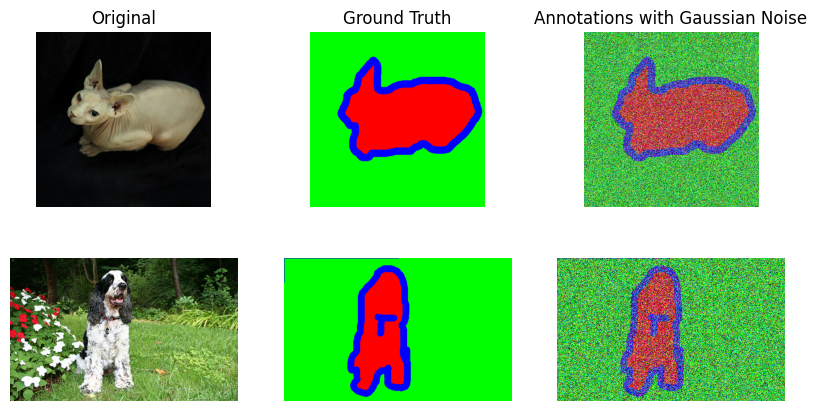
\includegraphics[width=0.7\textwidth]{Cap2/Figures/naive_gaussian_noise.png}
  \caption{Example of a noisy mask generated by naively introducing random
  noise into a ground truth mask. Morphological consistency is lost.}
  \label{fig:noisy_masks}
\end{figure}

For this reason, a more sophisticated approach was needed to create
datasets with emulated noisy annotations. The approach used here was
to use a pre-trained U-Net model to produce a good enough segmentation
of the image, which was then used to produce a ``noisy'' annotation by
introducing random noise into the last encoder layers of the model, thus
preserving the morphological consistency of the original annotation.
This strategy works since slight modifications introduced into
the encoder layers weights, somehow resemble conceptual disturbances with
respect to the original ground truth label, which kind of emulates
the cultural behavior of having a different interpretation of the
image, either for having a different level of expertise or for having a
different point of view or school of thought. The first encoding layers
were not modified, since it is expected human labelers would agree on the
most fundamental structures (analog to extracted features from initial
convolutional layers) in a similar way, thus preserving the morphological
consistency of the original annotation.

In this way, the level of ``disturbance'' with respect to the ground
truth for an emulated annotator can be controlled by the level of
noise introduced into the weights of the last encoder layers, thus:

\begin{equation}
  \mathbf{W}_{noisy} = \mathbf{W}_{original} + \mathcal{N}(0, \sigma^2)
\end{equation}

where $\mathbf{W}_{original}$ represents the original weights of the
last encoder layers, $\mathcal{N}(0, \sigma^2)$ is a Gaussian
distribution with mean 0 and variance $\sigma^2$, and
$\mathbf{W}_{noisy}$ are the resulting noisy weights. The variance
$\sigma^2$ controls the level of noise introduced, and thus the
degree of disturbance in the resulting segmentation masks.

\subsubsection{Oxford-IIIT Pet Dataset}

Using the techniques described above, the Oxford-IIIT Pet Dataset
\cite{ParkhiEtAl2012} was used to create a dataset with emulated noisy
annotations. The almost perfectly uniform distribution of the dataset classes
makes it an ideal playground dataset for testing segmentation models
with a high degree of confidence in the ground truth annotations, at
the same time that cats and dogs are a common sight in the daily life of
most people, making it easier to find a labeler that is able to annotate
the images with a high degree of accuracy, which facilitates model
initial debugging. Figure \ref{fig:oxford_iii_overview} shows an example
of the annotations in the original dataset.

\begin{figure}[h]
  \centering
  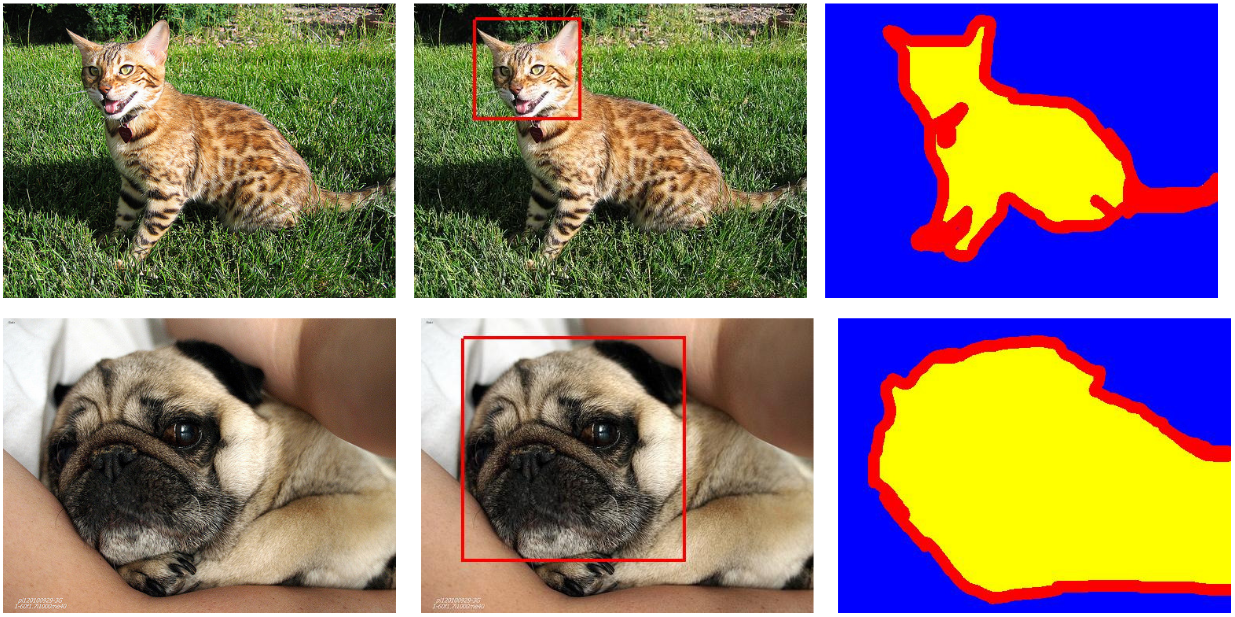
\includegraphics[width=0.7\textwidth]{Cap2/Figures/oxford_iii_overview.png}
  \caption{Annotations in the Oxford-IIIT Pet data. From left
    to right: pet image, head bounding box, and trimap segmentation
    (blue: background region; red: ambiguous region; yellow: foreground
  region).}
  \label{fig:oxford_iii_overview}
\end{figure}

With the application of the encoder layer weight perturbation technique,
the resulting noisy masks are shown in Figure
\ref{fig:enhanced_disturbances}. It can be seen that the
morphological consistency is preserved, even though the resulting
masks are far from the ground truth annotations, which goes perfectly
well for testing the robustness of the models against noisy
annotations in crowdsourcing-like scenarios.
\begin{figure}[h]
  \centering
  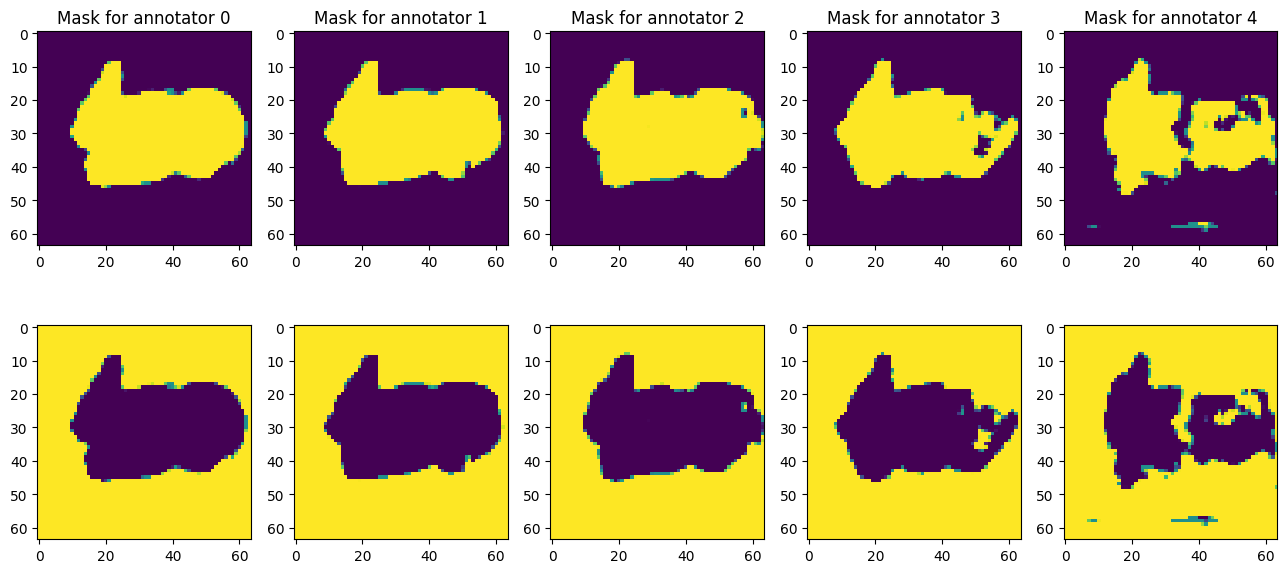
\includegraphics[width=0.8\textwidth]{Cap2/Figures/enhanced_disturbances.png}
  \caption{Noisy mask generated by enhancing the disturbances
    in the encoder layers weights for the Oxford-IIIT Pet Dataset.
    Morphological consistency is preserved. From left to right, SNR
  levels of noise in the encoder layer are 10, 5, 2, 0, -5 dB.}
  \label{fig:enhanced_disturbances}
\end{figure}

\subsection{Real histopathology datasets}

\subsubsection{Multi-Stain Breast Cancer Histological Dataset}

The Multi-Stain Breast Cancer Histological Dataset
\cite{WeitzEtAl2023} represents one of the largest publicly available
collections of whole slide images (WSIs) from surgical resection
specimens of primary breast cancer patients. This dataset is
particularly valuable for our work because it contains matched pairs
of H\&E and IHC-stained tissue sections from the same tumor, with a
total of 4,212 WSIs from 1,153 patients. The IHC stains include
important biomarkers such as ER, PGR, HER2, and KI67, which are
routinely used in breast cancer diagnosis and treatment planning
(more on staining techniques in Section \ref{sec:staining_techniques}).

The dataset's relevance to our work stems from several key aspects.
The matched H\&E and IHC stains allow for studying the consistency of
segmentation across different staining modalities, which is crucial
for understanding how different visualization methods affect
annotation quality. With 1,153 patients, the dataset provides a
robust foundation for training and evaluating segmentation models in
a real-world clinical setting. The inclusion of routine diagnostic
cases makes the dataset representative of actual clinical practice,
where variations in staining quality and tissue preparation are
common. Furthermore, the multiple biomarker stains (ER, PGR, HER2,
KI67) enable the study of how different tissue characteristics affect
segmentation performance and annotator agreement.

This dataset serves as an ideal testbed for our crowdsourced
segmentation approach. It allows us to evaluate how different
staining modalities affect annotator performance and agreement, while
also providing insights into the relationship between tissue
characteristics and segmentation difficulty. The dataset's
comprehensive nature enables validation of our models' performance
across different biomarker expressions and assessment of the
generalizability of our approach to real-world clinical data.

\begin{figure}[h]
  \centering
  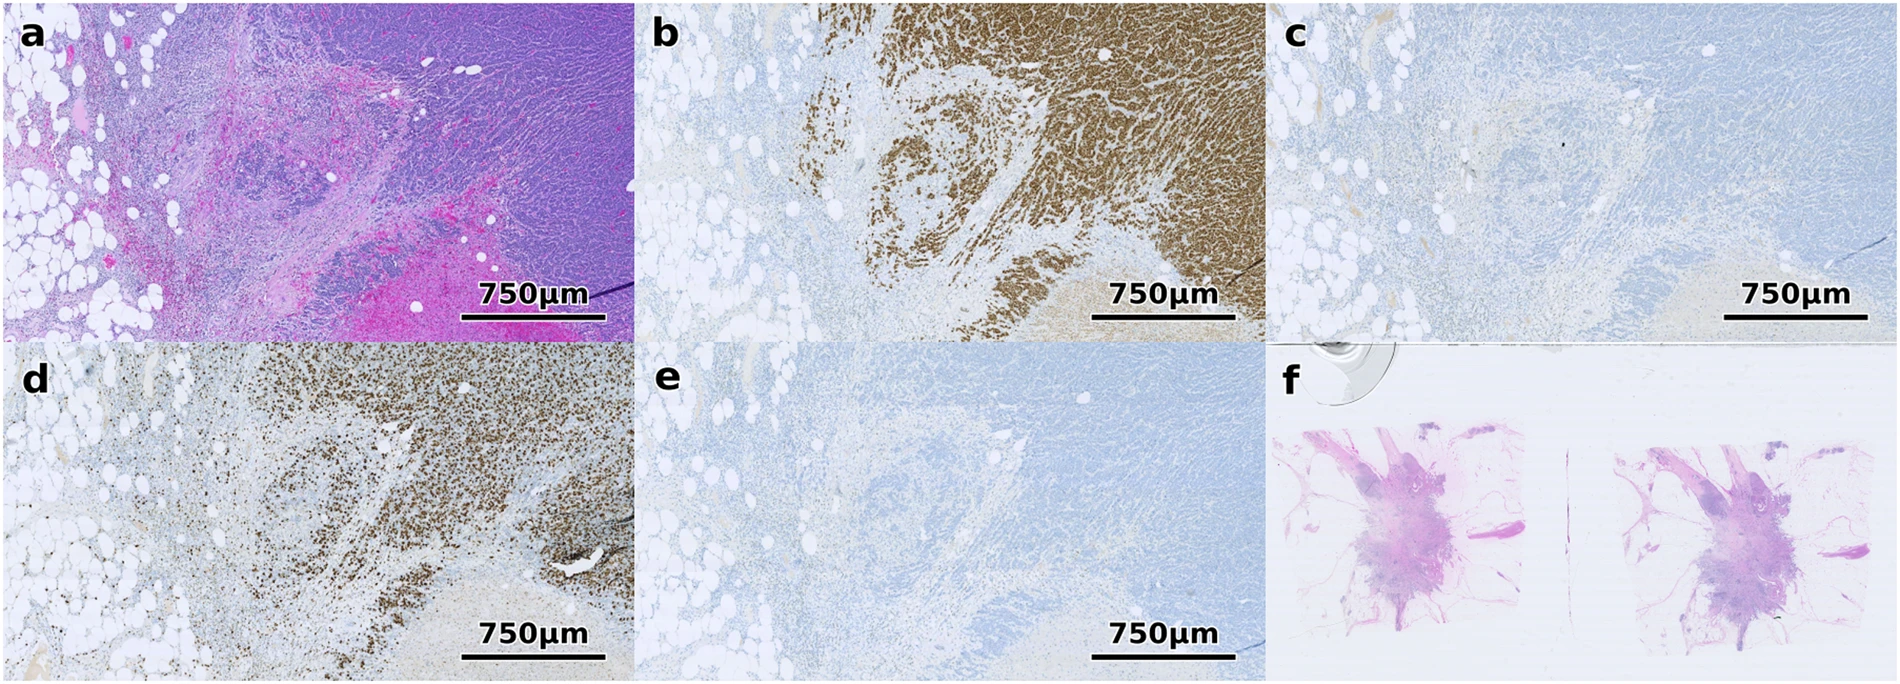
\includegraphics[width=0.7\textwidth]{Cap2/Figures/staining_comparison.png}
  \caption{Different staining techniques obtained from multi-stain
    breast cancer dataset \cite{WeitzEtAl2023}. (a) shows H\&E, (b) ER,
    (c) HER2, (d) Ki67 and (e) PGR. (f) shows an example of a \gls{WSI}
  that was excluded since it contains multiple tissue sections.}
  \label{fig:weitz_dataset_overview}
\end{figure}

\subsubsection{Structured Crowdsourcing Dataset for Histology Images}

The dataset presented by \cite{AmgadEtAl2019} is particularly
relevant to our work as it represents one of the first systematic
studies of crowdsourced annotations in histopathology. The authors
recruited 25 participants with varying levels of expertise (from
senior pathologists to medical students) to delineate tissue regions
in 151 breast cancer slides using the Digital Slide Archive platform,
resulting in over 20,000 annotated tissue regions.

Key aspects of this dataset make it valuable for our work. The
systematic evaluation of inter-participant discordance revealed
varying levels of agreement across different tissue classes, with low
discordance for tumor and stroma, and higher discordance for more
subjectively defined or rare tissue classes. The inclusion of
feedback from senior participants helped in curating high-quality
annotations, demonstrating that fully convolutional networks trained
on these crowdsourced annotations can achieve high accuracy (mean
AUC=0.945). The dataset also provides evidence that the scale of
annotation data significantly improves image classification accuracy.

This dataset is particularly valuable for our work because it
provides crucial insights into how annotator expertise affects
segmentation quality. It demonstrates the feasibility of using
crowdsourced annotations for training accurate segmentation models,
showing that even with varying levels of expertise, aggregated
annotations can produce reliable ground truth. The dataset includes a
systematic analysis of inter-annotator agreement, which is crucial
for understanding the challenges in crowdsourced histopathology
segmentation and informing the development of more robust
segmentation approaches.

\begin{figure}[h]
  \centering
  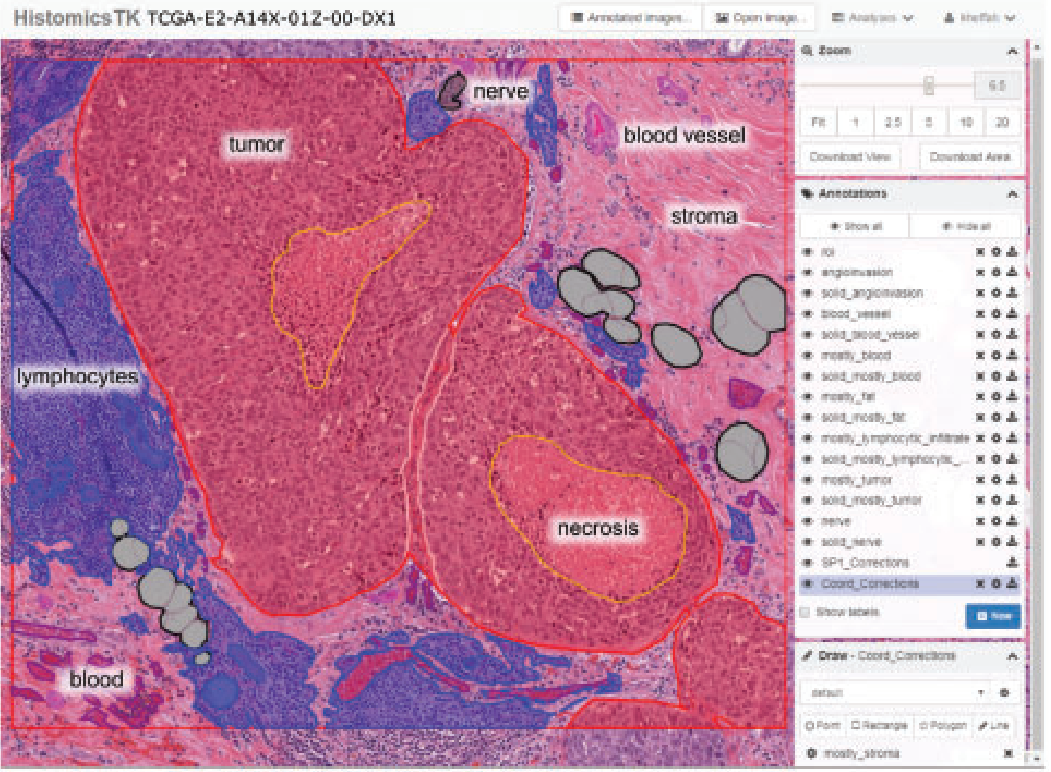
\includegraphics[width=0.8\textwidth]{Cap2/Figures/amgad_histomics_tk.png}
  \caption{Screenshot of the DSA and HistomicsTK web interface while
    creating the crowdsourced annotations for the dataset presented by
  \cite{AmgadEtAl2019}.}
  \label{fig:amgad_histomics_tk}
\end{figure}
